\documentclass{MUXLaTeX} % Versión 1.0.1 - Pruebas Beta - Pascal 2024

\usepackage{pgfgantt}
\usepackage{float}
\usepackage{tabularx}
\usepackage{graphicx}
\usepackage{array}
\usepackage{tabularx}
\usepackage{pdfpages}

\raggedbottom % El espacio sobrante queda en blanco al final de la pagina y no se reparte entre los bullets

\usepackage{enumitem}
\setlist{itemsep=0.2em, parsep=0pt, topsep=0.4em} % mismo espaciado para todas las listas

\selectlanguage{english}

\newcolumntype{P}[1]{>{\raggedright\arraybackslash}p{#1}}
\newcolumntype{Y}{>{\raggedright\arraybackslash}X}

\usepackage{pgfplots}
\pgfplotsset{compat=1.18}

\usepackage{listings}
\usepackage{xcolor}
\usepackage{tikz}
\usepackage{fvextra}
\usepackage{caption}

\lstdefinelanguage{Rust}{
  keywords={fn,let,mut,unsafe,if,else,while,for,in,const,impl,self,Self,
            as,use,pub,struct,trait,type,where,return},
  keywordstyle=\color{blue!60!black}\bfseries,
  ndkeywords={Vec,Arc,Complex,usize,f32,f64},
  ndkeywordstyle=\color{teal!70!black},
  comment=[l]{//},
  commentstyle=\color{gray}\itshape,
  morestring=[b]",
  stringstyle=\color{orange!70!black},
  sensitive=true
}
\lstdefinestyle{rustcode}{
  language=Rust,
  basicstyle=\ttfamily\footnotesize,
  numbers=left, numberstyle=\tiny\color{gray}, numbersep=8pt,
  frame=single, rulecolor=\color{black!25},
  backgroundcolor=\color{black!2},
  breaklines=true, columns=fullflexible, keepspaces=true,
  showstringspaces=false, tabsize=2, upquote=false,
  xleftmargin=1.5em, framexleftmargin=1.5em,
  escapechar=|
}
\newcommand{\cn}[1]{\tikz[baseline=(c.base)]\node[circle,draw,inner sep=0.7pt,font=\tiny\bfseries](c){#1};}

\DefineVerbatimEnvironment{JSONLog}{Verbatim}{
    fontsize=\footnotesize,
    breaklines=true,
    breakanywhere=true,
    breaksymbolleft={},
    breaksymbolright={},
    frame=none
}

\newcommand{\jsoncaption}[2]{%
    \begin{minipage}{\linewidth}
        \renewcommand{\lstlistingname}{Log}
        \captionof{lstlisting}{#1}
        \label{#2}
    \end{minipage}
}


\begin{document}
%%%%%%%%%%%%%%%% Elegir si / no (Minúsculas)
\bajavision{no} % no disponible en versión 1.0.1
\digital{no}
\abstract{si}
\indicetablas{si}
\indicefiguras{si}

%%%%%%%%%%%% PORTADA, ÍNDICE, RESUMEN
\maquetacion
{AtrilMatic: A Web-based Smart Music Stand} % TITULO
{\autoria{Tim Matveev y Elena Juarros}{Calificación final individual/Individual final grade: ??}} % AUTORÍA
{\direccion{Manuel Freire Morán}{no}{no}} % DIRIGIDO POR

%%%%%%%%%%%% CAPÍTULOS

\pagenumbering{arabic} % No borrar


\chapter{Introduction}

\section{Motivation}

\section{Objectives / goals ??}

\subsection{General objective}

\subsection{Specific objectives}

\section{Planning}

\chapter{Related work}

\section{Introduction}

\section{Technological foundations}

\section{Existing solutions}

Before starting with our own app, we felt that a way of gathering... 
was looking into already existing solutions in the market to see 
what we liked or not...??? 

This section reviews 3 applications that propose similar solutions to what 
we wanted to do. The solutions analysed are: Tomplay, Oktav and Newzik.

\subsection{Tomplay}

\todo[inline]{Review why citations are not appearing.}

Tomplay~\cite{tomplay} is a mobile and desktop app.

\begin{figure}[H]
	\centering
	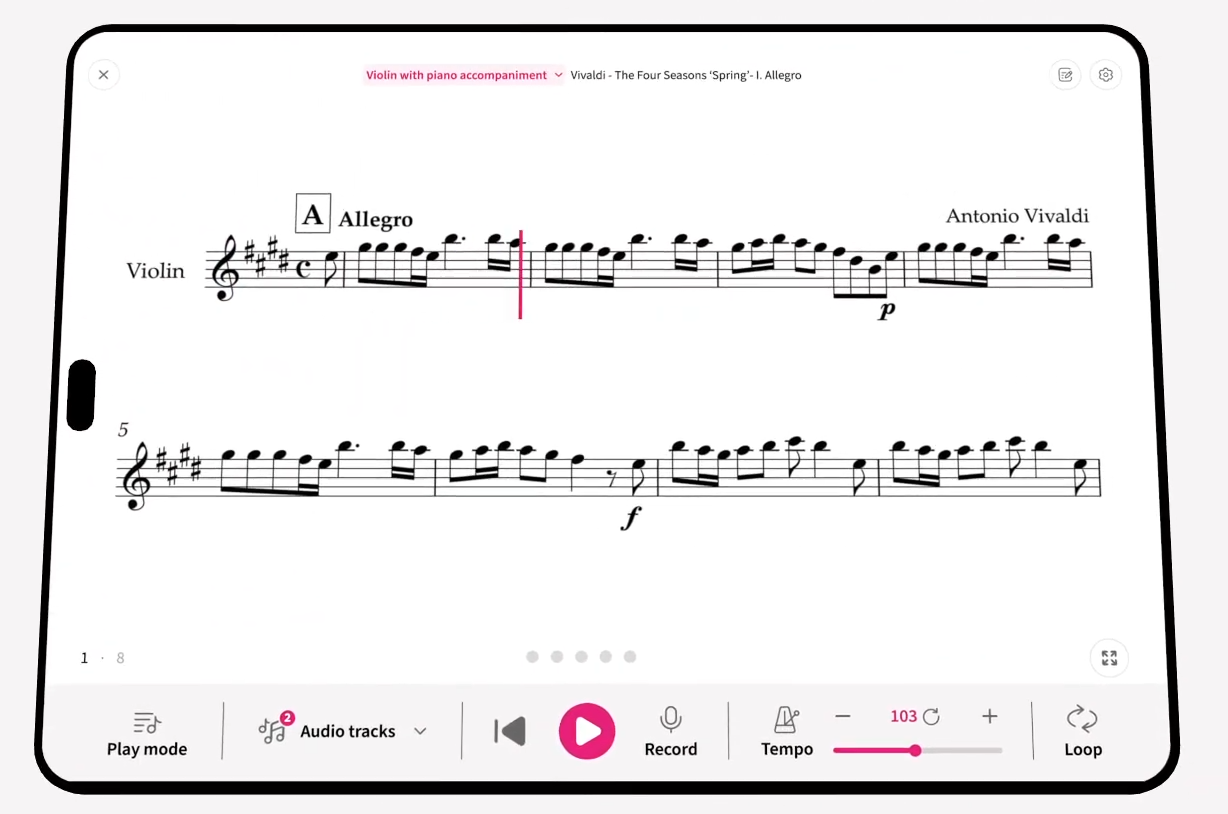
\includegraphics[width=0.6\textwidth]{Images/tomplay.png}
	\caption{Tomplay user interface.}
	\label{fig:tomplay}
\end{figure}

Its main features are:
\begin{itemize}
	\item \textbf{Digital sheet music}: Automatically scrolls in sync with the music.
	\item \textbf{Note by note practice}: The score advances only when you play the right note.
	\item \textbf{Adjust the tempo}: Slow down or speed up the music tempo.
	\item \textbf{Record yourself}: Record and listen back to your performance.
	\item \textbf{Annotate}: Add your own annotations to the music sheet.
	\item \textbf{Big music sheet catalogue}: Over 100,000 scores with professional audio accompaniments.
\end{itemize}

However, it presents some limitations:
\begin{itemize}
	\item Paid subscription
	\item 
	\item 
\end{itemize}

\todo[inline]{Add some more limitations.}


\subsection{OKTAV}

OKTAV~\cite{oktav} is a web app.

\begin{figure}[H]
	\centering
	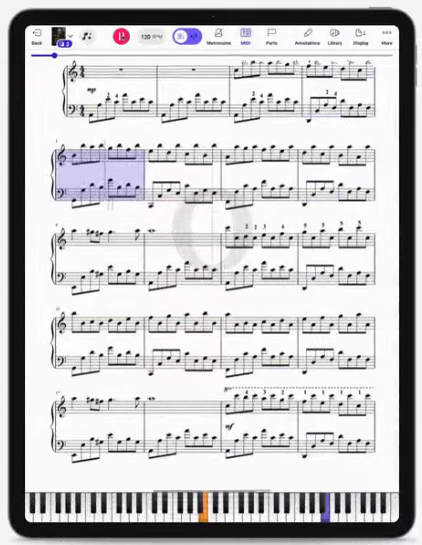
\includegraphics[width=0.4\textwidth]{Images/oktav.png}
	\caption{Oktav user interface.}
	\label{fig:oktav}
\end{figure}

Its main features are:
\begin{itemize}
	\item \textbf{Autoscroll}: Play without the need to turn pages and adjust tempo.
	\item \textbf{Annotate}: Ability to add fingerings, notes or highlight sections.
	\item \textbf{Play-along}: listen and play along to sheet music based on MIDI.
	\item \textbf{Digital piano}: See how to play a music sheet on a visual keyboard shown along the music sheet. 
\end{itemize}

Its limitations are:
\begin{itemize}
	\item Paid subscription
	\item Only for piano, violin and cello
	\item 
\end{itemize}

\subsection{Newzik}

Newzik~\cite{newzik}
is a web and mobile app.

\begin{figure}[H]
	\centering
	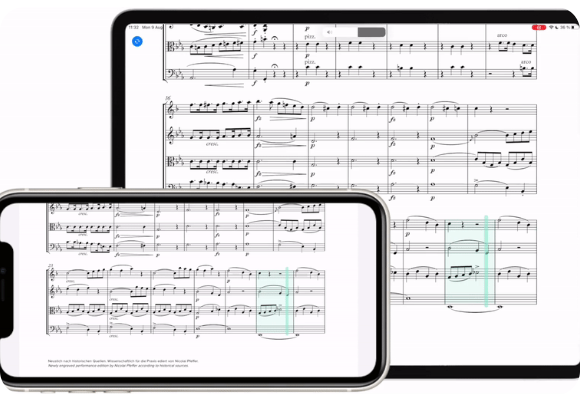
\includegraphics[width=0.6\textwidth]{Images/newzik.png}
	\caption{Newzik user interface.}
	\label{fig:newzik}
\end{figure}

Its main features are:
\begin{itemize}
	\item \textbf{Organization}: Centralize your digital sheet music (PDFs, scans, sets).
	\item \textbf{Play \& listen}: Listen to your sheet music with an AI that reads it for you.
	\item \textbf{Annotate \& turn pages}: Highlight, add fingerings and markers, and turn pages hands-free using facial movements (or a Bluetooth pedal).
\end{itemize}

Its limitations are:
\begin{itemize}
	\item Paid subscription
	\item Mobile app is only available for iOS
	\item No real-time tracking, you need to use gestures or a pedal to turn pages
\end{itemize}

\section{Comparison with the proposed solution}

Table~\ref{tab:existing-solutions} summarises the main characteristics of the solutions reviewed and our app.

\todo[inline]{Fill in the table below}

\begin{table}[H]
	\centering
	\begin{tabularx}{\textwidth}{l Y Y Y Y}
		\toprule
		\textbf{Feature} & \textbf{Tomplay} & \textbf{Oktav} & \textbf{Newzik} & \textbf{AtrilMatic} \\
		\midrule
		Platform			& Mobile and desktop	& Web 			& Web and iOS	& Web \\
		Price				& Paid 					& Paid 			& Paid 			& Free \\
		Score format		& Paid 					& Paid 			& Paid 			& PDF, MusicXML, XML \\
		Real-time tracking	& Paid 					& Paid 			& Paid 			& Yes \\
		Automatic page turn	& Paid 					& Paid 			& No 			& Yes \\
		Performance stats	& Paid 					& Paid 			& Paid 			& Not for now \\
		\bottomrule
	\end{tabularx}
	\caption{Comparison of existing solutions.}
	\label{tab:existing-solutions}
\end{table}
\chapter{Development}

\subsection{Functional requirements}

\subsection{Non-functional requirements}

\section{Design}

\subsection{Technical Challenges}



We commence by outlining the actual technological needs an
application like Atril would require. Recognizing pitch dynamically from
microphone input could, in general, be considered a resource-intensive and in
some ways non-deterministic task for a computer to perform. It is clear that
a system made to perform such a task should be capable of adjusting to
different microphones as well as different noise levels, and of recognizing
frequencies with a minimal margin of error. The fact that, in the case of
this application, such a task would have to be performed dynamically and in
real time would mean that it would prove to be even more challenging.
Furthermore, there is a prediction or matching element that uses the pitch
data produced by the recognition system to give the best possible estimate of
the position of the player in accordance with the musical composition being
played. It is important to highlight that this is probably where the biggest
technological focus should be allocated when it comes to an application like
Atril. The recognition and prediction logic will run multiple times a second
while also having to be lightweight and easy to implement into the vast world
of web development frameworks, languages, and established principles.

\subsection{WebAssembly}

WebAssembly seems to be ideal for this task. WebAssembly is a bytecode that
acts as a compilation target for many, usually low-level, programming
languages, famously C, C++, Rust, and Go. It offers simple validation, fast
compilation, and interoperability with the web platform, including direct
access to JavaScript and Web APIs~\cite{haas2017bringing}.

\subsection{Why WebAssembly?}
\label{sec:why-webassembly}

Although WebAssembly was initially widely adopted mostly as a platform for
cryptomining, this has since become a marginalized minority, comprising less
than 1\% of the binaries found on the web among the 8,461 WebAssembly
binaries studied by the University of Stuttgart in their 2021 paper
\textit{An Empirical Study of Real-World WebAssembly
Binaries}~\cite{hilbig2021empirical}, showing a wide adoption of the format
for a variety of use cases.

WebAssembly as a compilation target for the note recognition and prediction
system outlined earlier is a clear choice due to several important factors.
Firstly, it offers a low-overhead means of execution that will not bog down
or make the rest of the proposed application heavier. Additionally, it offers
a compilation target for languages that are significantly faster than
JavaScript, allowing the creation of a performant library that is still
entirely interoperable with the web world and its systems via a simple API
system. Finally, and importantly, WebAssembly is an abstraction over modern
hardware, meaning that our application will still remain platform
independent.

\subsection{Limitations and Solutions}

It is important to note the limitations of WebAssembly and the measures that
can be taken to minimize their impact. Hilbig et
al.~\cite{hilbig2021empirical}, in their study of 8,461 real-world binaries,
found that ``vulnerabilities that propagate from insecure source languages
potentially affect a wide range of binaries (e.g., two thirds of the binaries
are compiled from memory unsafe languages, such as C and C++)''. This matters
because WebAssembly's built-in safeguards do not neutralize such bugs. The
choice of source language, and its safety, is therefore crucial when
developing a WebAssembly system.

\subsection{Rust and WebAssembly}

Among the languages commonly compiled to
WebAssembly, Rust is the strongest candidate with respect to memory safety.
Rust's compiler enforces ownership and borrowing: a value has one owner, and
there can be either one mutable reference or many shared ones, never both.
For safe Rust, this rules out data races and invalid memory accesses, a
property that has been formally proven in machine-checked form for a
realistic subset of the language and for several core standard-library
abstractions~\cite{jung2018rustbelt}. Importantly, this is achieved without
garbage collection, whereas languages such as Go rely on runtime memory
checking and garbage collection~\cite{xu2022memory}. Rust's guarantees
therefore come largely from compile-time analysis rather than runtime
overhead, which is essential for a real-time audio application.

\subsection{WebAssembly Compilation Process}

\todo[inline]{MFM - Pictures are said to be worth a thousand words. Get a picture of the process.}

What follows is a small explanation of the WebAssembly compilation process,
sufficient to understand the functionality of our system. In our case, Rust
uses the LLVM intermediate representation, allowing a single intermediate
representation to be compiled to a variety of different targets. In this
case, LLVM has a WebAssembly target that converts the intermediate
representation given by the Low-Level Virtual Machine into a \texttt{.wasm}
module, a compact, stack-based bytecode in which high-level Rust constructs
such as structs and slices are lowered to a small set of primitive numeric
types and offsets into a linear memory, and in which control flow is
structured~\cite{haas2017bringing}. Because WebAssembly can only exchange
numbers with JavaScript directly, a tool such as \texttt{wasm-bindgen}
post-processes the module and generates the JavaScript and TypeScript glue
code that translates richer types such as strings and objects across the
boundary~\cite{wasmbindgen}. At load time, the browser engine validates the
module against WebAssembly's type system before executing anything, which is
what allows untrusted code to be run safely~\cite{haas2017bringing}. The
format was designed to be fast to validate and compile, and the engine then
translates it to machine code and runs it inside a sandbox that confines it
to its own linear memory~\cite{haas2017bringing}.

\subsection{System architecture overview}

\subsection{Database design -- we dont have DB!}

\section{Implementation}

\subsection{Backend and persistence}

\section{Key Algorithms}
\label{sec:key-algorithms}


\subsection{A Small Primer on Music Theory and its Physics}

Sound consists of pressure variations travelling through the air as a
longitudinal wave~\cite[\S1.1, pp.~1--2]{benson2006music}, so it obeys the
physics of waves. Much of music theory follows from this physics together
with the particular way the human ear perceives such waves. We therefore
start by relating the physical quantities of a sound to the musical
attributes we perceive (Table~\ref{tab:sound-attributes}).

\begin{table}[htbp]
  \centering
  \begin{tabular}{ll}
    \toprule
    Physical & Perceptual \\
    \midrule
    Amplitude & Loudness \\
    Frequency & Pitch    \\
    Spectrum  & Timbre   \\
    Duration  & Length   \\
    \bottomrule
  \end{tabular}
  \caption{Attributes of sound: physical quantities and the perceptual
  attributes they correspond to. Adapted from
  Benson~\cite[\S1.1, p.~2]{benson2006music}.}
  \label{tab:sound-attributes}
\end{table}

A larger amplitude of the pressure variation is perceived as a louder
sound, although perceived loudness also depends on frequency and is
measured on a logarithmic scale~\cite[\S1.3, pp.~9--11]{benson2006music}.
\emph{Pitch} is the perceived highness of a sound and corresponds
to its frequency, measured in hertz~\cite[\S1.1, p.~2; \S1.3, p.~8]{benson2006music}.
Perception is not identical to the physical signal: a pitch can be heard
at a frequency that is not actually present in the waveform (the
``missing fundamental'')~\cite[\S1.1, p.~2]{benson2006music}.

A \emph{tone} is a sound with a definite pitch, while a \emph{note} is a
named pitch in a musical system, such as A or C$\sharp$. In Western music
the octave is divided into twelve equal steps called
semitones~\cite[App.~M, p.~389]{benson2006music}. Two semitones make a
\emph{whole tone}, and the same word is also used for the interval
itself~\cite[App.~M, p.~389]{benson2006music}. Each semitone corresponds
to a frequency ratio of $2^{1/12}$, so twelve of them multiply the
frequency by exactly two.

An \emph{octave} is a doubling of frequency, for example from 220\,Hz to
440\,Hz~\cite[\S4.2, p.~137]{benson2006music}. Notes an octave apart are
perceived as playing equivalent roles in harmony and share the same note
name, a principle known as \emph{octave
equivalence}~\cite[\S4.2, pp.~137--138; App.~M, p.~389]{benson2006music}.
This is a consequence of the fact that our perception of musical distance
is logarithmic in frequency: musical intervals add, while the
corresponding frequency ratios multiply~\cite[\S5.4, p.~157]{benson2006music}.
A pitch of frequency $f$ is therefore measured relative to a reference
frequency $f_{\mathrm{ref}}$ by $\log_2(f/f_{\mathrm{ref}})$ octaves, or
$1200\log_2(f/f_{\mathrm{ref}})$ cents~\cite[\S5.4, p.~158]{benson2006music}.

\subsection{The algorithms used}

At the heart of detecting a pitch from time-domain data stands the Fast
Fourier Transform (FFT). In this project, the FFT is provided by the
\texttt{rustfft} crate~\cite{rustfft} and is combined with several
self-implemented window functions, which are discussed further below. The FFT
converts the time-domain data obtained from the microphone input into
frequency-domain data, which is then used by the pitch detection algorithms,
although some of them, such as the YIN algorithm, still work directly with
time-domain data.

\subsection{Fast Fourier Transform Algorithm}
\label{subsec:fft}

The Fourier transform is a mathematical operation that converts a signal,
given as an amplitude through time, into a spectrum in which each frequency
present in the signal is displayed together with its amplitude. It rests on
the Fourier series, which states that a periodic signal $f(t)$ with period
$T$ can be written as a sum of sine and cosine waves whose frequencies are
integer multiples of the fundamental frequency $\omega_0 = 2\pi/T$:
\begin{equation}
  f(t) = \frac{a_0}{2} + \sum_{n=1}^{\infty}
  \left[ a_n \cos(n\omega_0 t) + b_n \sin(n\omega_0 t) \right].
  \label{eq:fourier-series}
\end{equation}

Essentially, the Fourier transform shows which frequencies make up a given
signal and in which proportions. In effect, it determines how much of each
sine and cosine wave is needed to reconstruct the signal. To find how much of
frequency $F$ a signal contains, the signal is multiplied by a wave of
frequency $F$ and the average is taken. If the signal contains that
frequency, the product is mostly positive and the average is large.
Otherwise, the positive and negative parts cancel and the average is near
zero. Using a cosine copy and a sine copy makes the answer independent of the
phase of the wave. For the series above, this is exactly how the coefficients
are obtained:
\begin{equation}
  a_n = \frac{2}{T} \int_{0}^{T} f(t) \cos(n\omega_0 t)\, dt,
  \qquad
  b_n = \frac{2}{T} \int_{0}^{T} f(t) \sin(n\omega_0 t)\, dt.
  \label{eq:fourier-coefficients}
\end{equation}
Repeating this for every frequency yields the spectrum.

In practice, the microphone delivers a finite number $N$ of discrete samples
$x_0, \dots, x_{N-1}$, so the discrete Fourier transform (DFT) is used. With
the principal $N$th root of unity $W$ it can be written compactly
as~\cite{cooley1965algorithm}
\begin{equation}
  X_k = \sum_{n=0}^{N-1} x_n \, W^{kn},
  \qquad k = 0, 1, \dots, N-1,
  \qquad W = e^{-2\pi i / N}.
  \label{eq:dft}
\end{equation}
By Euler's formula,
$W^{kn} = \cos(2\pi kn/N) - i\sin(2\pi kn/N)$, so
Equation~\ref{eq:dft} multiplies the signal by a cosine copy and a sine copy
and sums the result, which is the discrete counterpart of the averaging
described above. Bin $k$ corresponds to the frequency $f_k = k f_s / N$,
where $f_s$ is the sampling rate, and the magnitude $|X_k|$ gives the
strength of that frequency in the signal.

Evaluating Equation~\ref{eq:dft} directly requires on the order of $N^2$
operations. The FFT is not a different transform but a fast way of computing
this one: the algorithm of Cooley and Tukey needs, in their words, ``a number
of operations proportional to $N \log N$ rather than $N^2$''%
~\cite{cooley1965algorithm}. This difference is what makes it feasible to run
the analysis several times per second on live microphone input. In the
current implementation, the sample rate is 48\,kHz, the FFT and window sizes
are 2048 samples, and the hop size is 512 samples, so a new spectrum is
computed every 512 samples, approximately 94 times per second.

\subsection{SIMD radix-4 FFT in RustFFT}
\label{sec:simd-radix4}

Listing~\ref{lst:radix4-pass} shows the core of the WebAssembly SIMD
radix-4 FFT in RustFFT 6.4.1~\cite{rustfft} (excerpt of
\texttt{wasm\_simd\_radix4.rs}, lightly shortened), and
Listing~\ref{lst:butterfly4} the underlying four-point butterfly
(\texttt{wasm\_simd\_vector.rs}).

\begin{lstlisting}[style=rustcode,
  caption={Layered radix-4 pass of the WASM SIMD FFT (excerpt).},
  label={lst:radix4-pass}]
#[target_feature(enable = "simd128")]
unsafe fn perform_fft_immut(&self, input: &[Complex<T>],
                            output: &mut [Complex<T>], _scratch: &mut [Complex<T>]) {
    // |\cn{1}| digit-reversed copy, so every sub-FFT is contiguous
    if self.len() == self.base_len {
        output.copy_from_slice(input);
    } else {
        bitreversed_transpose::<Complex<T>, 4>(self.base_len, input, output);
    }

    // |\cn{2}| N / base_len small FFTs, one per contiguous chunk
    self.base_fft.process_with_scratch(output, &mut []);

    // |\cn{3}| merge four FFTs of length L into one of length 4L, layer by layer
    const ROW_COUNT: usize = 4;
    let mut cross_fft_len = self.base_len * ROW_COUNT;
    let mut layer_twiddles: &[S::VectorType] = &self.twiddles;

    while cross_fft_len <= input.len() {
        let num_rows = input.len() / cross_fft_len;
        let num_scalar_columns = cross_fft_len / ROW_COUNT;
        let num_vector_columns =
            num_scalar_columns / S::VectorType::COMPLEX_PER_VECTOR;

        for i in 0..num_rows {                      // independent chunks
            butterfly_4::<S, T>(                    // |\cn{4}| all columns, in place
                &mut output[i * cross_fft_len..],
                layer_twiddles, num_scalar_columns, &self.rotation)
        }

        let twiddle_offset = num_vector_columns * (ROW_COUNT - 1);
        layer_twiddles = &layer_twiddles[twiddle_offset..];
        cross_fft_len *= ROW_COUNT;
    }
}
\end{lstlisting}

\begin{lstlisting}[style=rustcode,
  caption={Four-point column butterfly on SIMD vectors (\texttt{f64} case).},
  label={lst:butterfly4}]
unsafe fn column_butterfly4(rows: [Self; 4], rotation: Rotation90<Self>) -> [Self; 4] {
    // |\cn{5}| first stage: sums and differences of rows (0,2) and (1,3)
    let [mid0, mid2] = Self::column_butterfly2([rows[0], rows[2]]);
    let [mid1, mid3] = Self::column_butterfly2([rows[1], rows[3]]);

    // multiplication by -i: lane swap and sign flip, no multiplication
    let mid3_rotated = Self::apply_rotate90(rotation, mid3);

    // |\cn{6}| second stage, returned in natural frequency order
    let [output0, output1] = Self::column_butterfly2([mid0, mid1]);
    let [output2, output3] = Self::column_butterfly2([mid2, mid3_rotated]);
    [output0, output2, output1, output3]
}
\end{lstlisting}

\paragraph{How the transform is computed in parallel.}
After the digit-reversed copy \cn{1} and the small base transforms \cn{2},
each layer \cn{3} views a block of $4L$ values as a $4 \times L$ grid whose
rows are four already-finished FFTs of length $L$. The columns of this grid
are mutually independent, so \cn{4} can process all of them with the same
instruction sequence: each column is multiplied by its twiddle factors
$W_{4L}^{jm}$ and fed through the four-point butterfly \cn{5}\cn{6}, which
consists only of additions, subtractions and a free rotation by $\pm i$.
On WebAssembly this sequence runs on 128-bit \texttt{v128} registers: one
instruction operates on a whole vector of complex numbers (one \texttt{f64}
or two \texttt{f32} values per vector), so the real and imaginary parts, and
for \texttt{f32} two neighbouring columns, are updated simultaneously.
Together with the $\log_4 N$ layers and the independent blocks inside each
layer, this data-parallel structure is what lets the FFT use WebAssembly SIMD
efficiently.

\subsection{Window Functions}
\label{subsec:win-func}

When computing the FFT, the algorithm behaves as if it were being applied to
a spectrum that repeats infinitely. A wave that is cut off at the edge of the
block therefore creates a noticeable elevation in amplitude which skews the
results. This phenomenon is called spectral leakage. To reduce it, different
window functions are applied to the signal before the FFT is computed. The
general idea behind all window functions is to fade the edges of the block,
although this is achieved through different means. The error can be reduced
by multiplying the block with a window function $w[n]$ that fades the signal
towards zero at both ends before the transform is computed:
\begin{equation}
  y[n] = w[n]\, x[n], \qquad n = 0, 1, \dots, N-1.
  \label{eq:windowed-signal}
\end{equation}
Every window is a compromise between two properties of its spectrum: the width
of the main lobe, which determines how close two frequencies can be before
they blur into one, and the height and decay of the side lobes, which
determine how much a strong component leaks into its surroundings
\cite{harris1978windows}. The four windows used in this project all belong to
the family of cosine-sum windows,
\begin{equation}
  w[n] = \sum_{m=0}^{M} (-1)^m a_m \cos\!\left( \frac{2\pi m n}{N-1} \right),
  \qquad n = 0, 1, \dots, N-1,
  \label{eq:cosine-sum}
\end{equation}
and differ only in the number of terms and in the coefficients $a_m$.

\subsubsection{Rectangular Window}

The rectangular window does not modify the signal at all ($M=0$,
$a_0=1$):
\begin{equation}
  w_{\mathrm{R}}[n] = 1.
  \label{eq:rect}
\end{equation}
It has the narrowest main lobe of the four, so it separates close
frequencies best, but its side lobes are the highest and decay slowly. It is
only a good choice when the signal is guaranteed to be periodic within the
block.

\subsubsection{Hann Window}

The Hann window is a single raised cosine ($M=1$, $a_0=a_1=0.5$) that
reaches exactly zero at both ends of the block:
\begin{equation}
  w_{\mathrm{Hann}}[n] = 0.5 - 0.5 \cos\!\left( \frac{2\pi n}{N-1} \right).
  \label{eq:hann}
\end{equation}
Because the block ends at zero, the repeated copies join smoothly, and the
side lobes are low and fall off quickly. The price is a main lobe twice as
wide as that of the rectangular window.

\subsubsection{Hamming Window}

The Hamming window uses the same shape with different coefficients
($a_0=0.54$, $a_1=0.46$):
\begin{equation}
  w_{\mathrm{Hamming}}[n] = 0.54 - 0.46 \cos\!\left( \frac{2\pi n}{N-1} \right).
  \label{eq:hamming}
\end{equation}
These are the commonly used rounded values of the coefficients. The window
does not quite reach zero at the ends, which lowers the nearest side lobes
further than the Hann window does, but a small discontinuity remains, so the
distant side lobes decay slowly.

\subsubsection{Blackman Window}

The Blackman window adds a second cosine term ($M=2$, $a_0=0.42$,
$a_1=0.5$, $a_2=0.08$):
\begin{equation}
  w_{\mathrm{Blackman}}[n] = 0.42 - 0.5 \cos\!\left( \frac{2\pi n}{N-1} \right)
  + 0.08 \cos\!\left( \frac{4\pi n}{N-1} \right).
  \label{eq:blackman}
\end{equation}
It gives the lowest leakage of the four and its side lobes fall off quickly,
at the cost of the widest main lobe. It is useful when a weak component has to
be found next to a much stronger one.

\subsubsection{Comparison}

Table~\ref{tab:windows} summarizes the trade-off. The main lobe width is
measured in FFT bins, where one bin corresponds to a frequency step of
$f_s/N$. The coherent gain is the mean value of the window,
$\frac{1}{N}\sum_{n=0}^{N-1} w[n]$; since the windowed signal is scaled by
this factor, amplitudes read from the spectrum must be divided by it.
\begin{table}[htbp]
  \centering
  \small
  \begin{tabular}{lcccc}
    \toprule
    Window & Main lobe width & Highest side lobe & Side-lobe decay & Coherent gain \\
           & (bins)          & (dB)              & (dB/octave)     &               \\
    \midrule
    Rectangular & 2 & $-13$ & 6  & 1.00 \\
    Hann        & 4 & $-31$ & 18 & 0.50 \\
    Hamming     & 4 & $-43$ & 6  & 0.54 \\
    Blackman    & 6 & $-58$ & 18 & 0.42 \\
    \bottomrule
  \end{tabular}
  \caption{Approximate properties of the four windows. The main lobe width is
  the distance between the first nulls on both sides of the peak.}
  \label{tab:windows}
\end{table}

\chapter{Evaluation}
\label{chap:evaluation}

The evaluation has two parts, a technical evaluation of pitch detection 
and score following, and a user evaluation.

\section{Objectives}

\begin{itemize}
	\item Measure how accurately each pitch detection algorithm identifies notes.
	\item Find the configuration (algorithm, window, FFT size) that works best.
	\item Check that the cursor follows the musician correctly.
	\item Assess the usability of the applicatin with real users.
\end{itemize}

\section{Technical evaluation}

\subsection{Test environment}
\label{subsec:test-env}

We built a browser-based test bench to compare algorithms and configurations 
under the same conditions. It runs the same WebAssembly module as the application.
Each test is a JSON file with an input, an expected result, and optionally its 
own configuration. The bench can run two configurations side by side on the same 
tests.

\todo[inline]{Add screenshot of the test bench.}

\subsection{Test types}

\begin{itemize}
	\item \textbf{Pitch detection:} synthetic sine waves at known frequencies, from a 
	single note (A4, 440\,Hz) to all 120 notes from C0 to B9.
	\item \textbf{Audio recognition:} real instrument recordings with a known sequence 
	of notes. \todo[inline]{add some more details (instruments use, etc)}
	\item \textbf{Score tracking:} checks that the cursor ends at the expected position 
	of the score, within a tolerance. \todo[inline]{add some more details}
\end{itemize}

The score-following logic is also covered by unit tests in Rust. They check that the 
cursor moves to each played note, stays still when the input is silent, ignores notes 
that are not in the score, skips rests and stops at the end of the score.

\subsection{Configurations}

\todo[inline]{Add table comparing configurations, link to algorithms section, 
maybe a screenshot of test bench}

\subsection{Metrics}

\todo[inline]{table explaining the metrics used}

\subsection{Results}

\todo[inline]{explain test bench results, add screenshots of test bench}

\section{User evaluation}

\subsection{Participants}

[Number, instrument, level, age range]

\subsection{Evaluation tasks}

[What each participant does (load a score, play, ...)]

\subsection{Procedure}

[Where, how long, devices used, ...]

THe questionnaire is in Appendix~\ref{ap:cuestionario}

\subsection{Results}

\section{Discussion}

[Findings and limitations of the evaluation]

\chapter{Conclusions}

\section{Conclusions}

\subsection{Fulfilment of the objectives / goals ??}
\begin{otherlanguage}{spanish}

\setcounter{chapter}{0}
\setcounter{section}{0}

\chapter{Introducción}

\section{Motivación}

\subsection{Objetivo general}

\subsection{Objetivos específicos}

\end{otherlanguage}
\begin{otherlanguage}{spanish}

\chapter{Conclusiones}

\section{Conclusiones}

\end{otherlanguage}

%%%%%%%%%%%% BIBLIOGRAFÍA AUTOMÁTICA
\bibliografia
\cleardoublepage
\appendix

\newcommand{\capituloapendice}[2]{%
    \refstepcounter{chapter}%
    \chapter*{\appendixname \thechapter\\[0.5ex]#1}%
    \phantomsection
    \addcontentsline{toc}{chapter}{\appendixname \thechapter: #1}%
    \markboth{\appendixname \thechapter: #1}{\appendixname \thechapter: #1}%
    \label{#2}%
}

\capituloapendice{Evaluation questionnaire}{ap:cuestionario}

This appendix presents ... 
\end{document}